% chap2.tex (Definitions)

\chapter{Background and Related Work}\label{background}

This section outlines some of the state of the art in the area of data provenance for file systems, data compression techniques for data provenance, and provenance-aware intrusion detection systems.

\section{Overview of Provenance Aware systems}

There has been a considerable amount of work done on data provenance collection. Some of this work has been focused on databases, sensor networks and system level provenance but so far little attention has been given to provenance in IoT devices. Some the previous work done on data provenance collection systems are outlined below:

\subsection{Provenance Aware Storage System(PASS)}
MuniswamyReddy
et al developed a provenance aware system that tracks  system level provenance of the linux file system.\textcolor{red}{ There are two versions PASS v1 and PASS v2. v1 allows... while version 2...} Provenance information
is stored in the same location as the file system for easy accessibility, backup,
restoration, and data management. Provenance information is collected and stored in
the kernel space. PASS is composed of 3 major components: provenance collector, and provenance storage, provenance query.The collector keeps track of system level provenance. It intercepts system calls which are translated into provenance data and initially stored in memory as inode catche. This provenance data is then transfered to a file system in an kernel database, BerkleyDB. This database maps key value pairs for provenance data for fast index look up. It also provides functionalities for querying provenance data in the database. The query tool is built ontop of Berkley DB. For querying, users can process queries using the provenance explorer. Query is done using commands such as MAKEFILE  GENERATION which creates the sequence of events that led to the final state of a file or process. DUMP ALL, gets the provenance of the requested file.PASS stores a refrence to the executable that created the provenance data, input files, A description of hardware in which provenance data is produced, OS information, process environment, process parameters, and other/data such as a random number generator seed.PASS detects and eliminates cycles that might occur in provenance dependencies as a result of version avoidance.Cycles violates the dependency relationships between entities. For example, a child node could depend on a parent node and also be an ancestor of a parent node. PASS eliminates cycles by merging processes that might have led to the cycles. 

\subsection{HiFi}
Bates et al. [2] developed system level provenance information for the Linux kernel using Linux Provenance Modules(LPM), which tracks at whole system provenance including interprocess communication, networking, and kernel activities. This is achieved by mediating access to kernel objects. Linux Security Model is a framework that was designed for providing custom access control into the Linux kernel.It consists of a set of hooks which is executed before access decision is made.LSM was designed to avoid problem created by direct system call interception. The provenance information from the kernel space is securely transmitted to the provenance recorder in the user space. 
\par HiFi contains three components, provenance collector, provenance log and provenance handler. The collector and log are contained in the kernel space while the handler is contained in the user space.The log is a storage medium which transmits the provenance data to the user space.The collector contains the LSM which resides the kernel space. The collector records provenance data and writes it to the provenance log.The handler intercepts the provenance record from the log.\textcolor{red}{This approach to collecting provenance data differs from our work since we focus on embedded systems and are concerned with input and output (I/O) data, which primarily involve sensor and actuator readings.}

\subsection{RecProv}

RecProv is a provenance system which records user level provenance, avoiding the overhead incurred by kernel level provenance recording.It uses mozilla rr to perform deterministic record and replay by monitoring system calls  and non deterministic input.Mozilla rr is a debugging tool for linux browser. It is developed for the deterministic recording and replaying of firefox browser in linux. It also ensure the integrity of provenance data up till the point at which a host is compromised by trace isolation. Mozilla rr relies on PTRACE which intercepts system calls during context switch.It uses PTRACE to monitor the CPU state ducring and after a system call. System calls such as execve, clone, fork, open, read, write, clode, dup, mmap, socket, connect, accept are monitored which is used for file versioning. the provenance information generated in converted into PROV-JSON a W3C standard for relaying provenacne information and also stores provenance data in Neo4j a graph database for visualization of provenance graphs and storage.It does not require changes to the kernel like most provenance monitoring systems (include citations of other provenance monitoring systems that require kernel modification). 

Recprov uses PTRACE\_PEEKDATA from PTRACE to access the derefrenced address of the traced process from the registers. 

\subsection{StoryBook}
Spillance et al developed a user space provenance collection system, Storybook \cite{Rabinovich1995}  that allows the collection of provenance data from the user space thereby reducing performance oververhead from kernel space provenance collection. This system is modular.It allows the use of application specific extensions allowing additions such as database provenance, system provenance, and web and email servers. It achieves provenance capture by using FUSE for system level provenance and MYSQL for database level provenance capture. StoryBook allows developers to implemement provenance inspectors. these are custom provenance models which captures the provenance of specific applications which are often modified by different application(e.g web servers, databases). When an operation is performed on a data object, the appropriate provenance model is triggered and provenance data for that data object is captured. SotryBook stores provenance information such as open, close, read or write, application specific provenance, causality relationship between entities contained in the provenance system(?). Provrenance is stored in key value pairs and It uses Fable as the storage backend. Storybook allows for provenance query.It achieves this by looking up inode in the file, ino hashtable.

\subsection{Trustworthy whole system provenance for Linux kernel}

Bates et al provide a security model for provenance collection in the linux kernel. This is achieved by creating a Linux Provenance Model(LPM). LPM serves as a security layer that provides a security abstraction for provenance data. It is involved in the attestation disclosure of the application layer, authentication channel for the network layer.The goal of LPM is to provide an end to end provenance collection system. 

LPM ensures the following security guarantees: for LPM,the system must be able to detect and avoid malicous forgery of provenance data. The system must be trusted and easily verifiable. 

\par When an application invokes a system call, the LPM tracks system level provenance which is transmitted to the Provenance module via the relay buffer . The provenance module registers contains hooks which records system call events. These events are sent to a provenance recorder in the user space. The provenance recorder ensures that the provenance data is sored in the appropriate backend of choice. Proveance recorders offer storage for Gzip, PostGreSQL, Neo4j and SNAP.



\subsection{Towards Automated Collection of Application-Level Data Provenance}
Tariq et all developed a provenance collection system which automatically collects the provenance of applications source code at run time. It takes a different approach from system level provenance capture. It achieves provenance capture by using LLVM compiler framework and SPADE provenance management system. LLVM is a framework that allows dynamic compilation techniques of applications written in C, C++, Objective-C, and Java.Provenance is inserted during compilation.LLVM contains an LLVM Reporter. This is a java class that parses the output file collected from the LLVM Tracer and forwards the provenance data collected to the SPADE Tracer. SPADE is a provenance management tool that allows for the tranformation of domain specific activity into provenance data. The LLVM Tracer module tracks provenance at the exit and entry of each function. The output is an Open Provenance Model in which functions are represented by an OPM process, arguments and return values are represented as an OPM artifact. To minimize provenance record, users are allowed to specify what functions they would like to collect provenance information at run time. The system discards provenance data that are not needed. This does not provide a whole system provenance of all activities that occurs on the system.The LLVM optimizer generates a graph of the target application. This graph is used to perform reverse reachability analysis  from the functions contained in the graph. 


A workflow of how the framework works in collecting provenance is as follows:

\begin{itemize}
\item The application is compiled and converted into bitcode using the LLVM C compiler, clang.

\item The LLVM Tracer module is compiled with the bitcode.

\item Provenance instrumentation is added to the bitcode via the LLVM Trace module.

\item instrumentation bitcode is converted into assembly code via the compiler llc

\item LLVM Tacer and Reporter is compiled into assembly code.

\item  The instrumented application and assembly code is compiled into an executable binary and sent to the SPADE kernel.
\end{itemize}

One major limitation to this approach of collecting application level provenance is that a user is required to have the source code of the specific application in which provenance data is required.Also, provenance collection is limited to function's exit and entry points.






\subsection{user space provenance with Sandboxing}
\textcolor{red}{TODO}


\subsection{Provenance for Sensors}
Lim et al. developed a
model for calculating the trust of nodes contained in a sensor network by using data
provenance and data similarity as deciding factors to calculate trust. The value of
provenance signifies that the more similar a data value is, the higher the trust score.
Also, the more the provenance of similar values differ, the higher their trust score.
This work differs from our approach since the authors focus on creating a trust score
of nodes connected in a sensor network using data provenance and do not emphasize
how the provenance data is collected. We are focused on creating a secure
provenance aware system for I/O operations which is used to ensure trust of
connected devices.




\section{Model for representing provenance for IoT}

In order to generate provenance, we need to satisfy the who, where, how, and what of data transformations.Provenance data is represented using a provenance model which is serialized as a JSON output. This model contains information such as sensor readings, device name, and device information. This information is mapped into an appropriate provenance data model  to allow for interoperability and visualization.

\subsection{Open Provenance Model(OPM)}

Open provenance model is a specification that was derived as a result of a meeting at the International Provenance and Annotation Workshop (IPAW) workshop in May 2006. OPM was created to address the need of allowing a unified way of representing provenance data amongst various applications. It allows for interchangeability between various provenance models that might exist. The goal of OPM is to develop a digital representation of provenance for entities regardless of if it is produced by a computer system or not. 

An example of such is depicted in Figure 7. This OPM graphs represents a process of driving a car.  \textcolor{red}{TODO: work on OPM Example}



OPM is represented as a directed acyclic graph which denotes causal dependency between entities. The edges in the graph denotes dependencies with its source denoting effect and its destination denoting cause.The definitions of the edges and their relationships are denoted below: 


\begin{itemize}
\item wasGeneratedBy: Shows relationship in which an entity(e,g artifact) is utilized by one or  more entities(e.g process). An entity can use multiple enities so it is important to define the role.  
\item wasControlledBy: This denotes a relationship in which an entity caused the creation of another entity.
\item used(Role): Denotes an enity requires the services of another enity in order to execute.
\item wasTriggeredBy: This relationship represents a process that was triggered by another process
\item wasDerrivedFrom: This relationship indicates that the source needs to have been generated before the destination is generated.
\end{itemize}

 There are three entities contained in the OPM model: artifact, process, agent. 

\begin{itemize}
\item
artifact: This represents the state of an entity.An artifact is graphically represented by a circle.

\item
Process: A process is an event which is taking place.A process is represented by a square object.

\item 
Agent: Agents are actors that facilitate the execution of a process.An agent is represented by a hexagon in an OPM graph.
\end{itemize}

OPM denotes all previous and current actions that have been performed on an entity and  the relationship between each entities contained in the graph. Figure 2 represents an example of an OPM acyclic graph with all of its causal dependencies. The goal of OPM is to be able to model the state of how things both digital or physical are at a given state.   

\begin{figure}[h]
\begin{center}

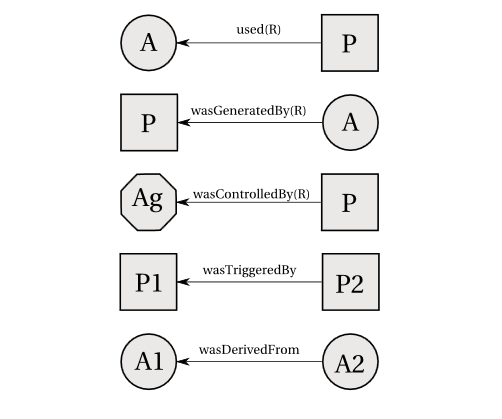
\includegraphics{opm_convention.PNG}
\end{center}
\caption{Edges and entities in OPM}
\label{autom}
\end{figure}

%\begin {center}
%\begin {tikzpicture}[-latex ,auto ,node distance =4 cm and 5cm ,on grid ,
%semithick ,
%state/.style ={ circle ,top color =white , bottom color = processblue!20 ,
%draw,processblue , text=blue , minimum width =1 cm}]
%\node[state] (C)
%{$1$};
%\node[state] (A) [above left=of C] {$0$};
%\node[state] (B) [above right =of C] {$2$};
%\path (A) edge [loop left] node[left] {$1/4$} (A);
%\path (C) edge [bend left =25] node[below =0.15 cm] {$1/2$} (A);
%\path (A) edge [bend right = -15] node[below =0.15 cm] {$1/2$} (C);
%\path (A) edge [bend left =25] node[above] {$1/4$} (B);
%\path (B) edge [bend left =15] node[below =0.15 cm] {$1/2$} (A);
%\path (C) edge [bend left =15] node[below =0.15 cm] {$1/2$} (B);
%\path (B) edge [bend right = -25] node[below =0.15 cm] {$1/2$} (C);
%\end{tikzpicture}
%\end{center}

\subsection{Provenance Data Model(Prov-DM)}

PROV-DM is a W3C standardized extension of OPM. Prov-DM is a model that is used for depict causal relationship between entities, activities and , and agents(digital or physical).  It creates a common model that allows for interchange of provenance information between heterogeneous devices. It contains two major components: types and relations. Figure below shows an example of a causal relationship between an entity, agent, and activity in a PROV-DM

%\begin{figure}[h]
%\begin{center}
%
%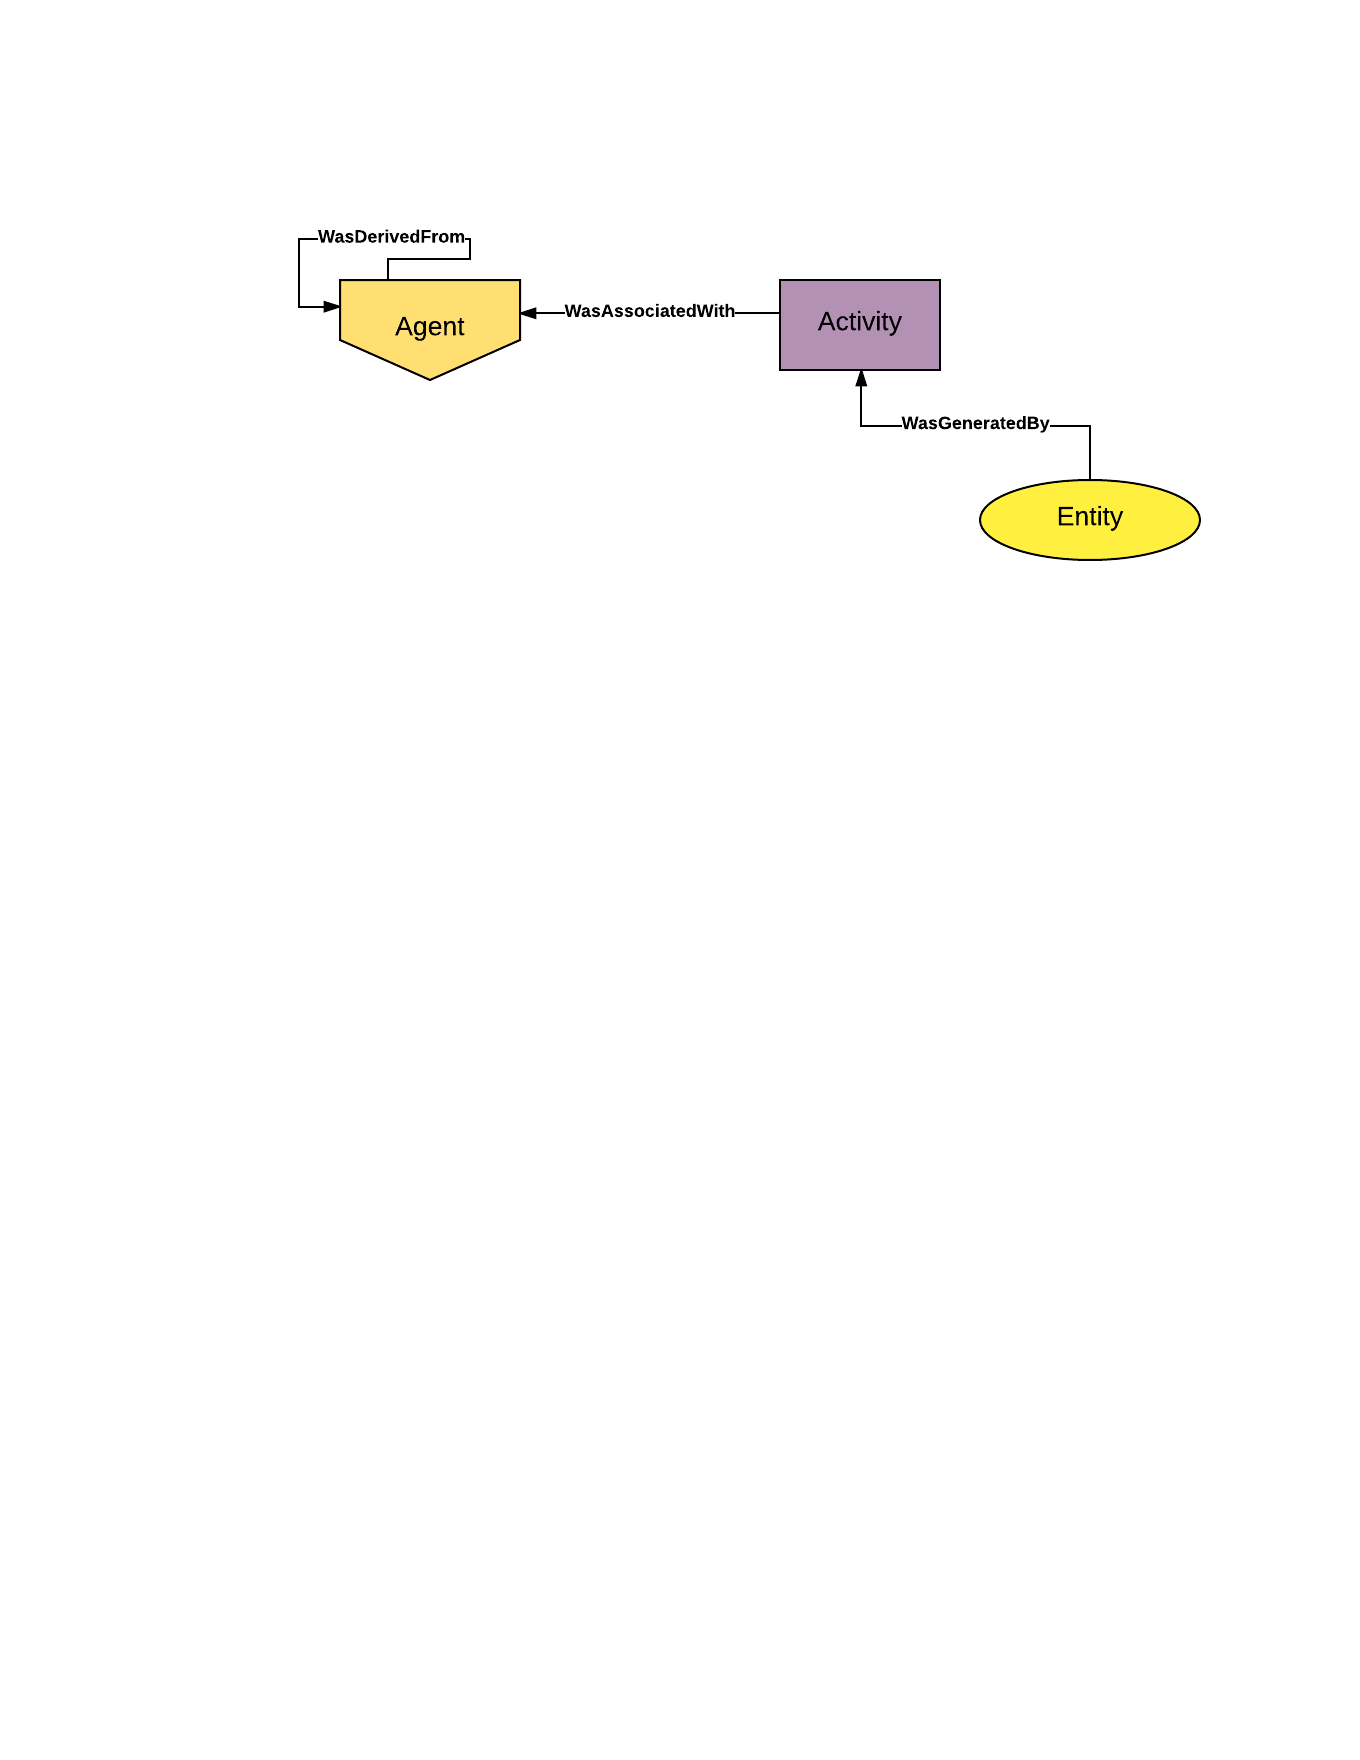
\includegraphics[height=7in]{prov_dm.PNG}
%\end{center}
%\caption{Prov DM}
%\label{autom}
%\end{figure}
%
\begin{itemize}

\item entity: An entity is a physical or digital object. An example of an entity is a file system, a process, or an motor vehicle.

\item Activity: An activity represents some form of action that occurs over a time frame.Actions are acted upon by an entity. an example of an activity is a process opening a file directory, Accessing a remote server.

\item Agent: An agent is a thing that takes ownership of an entity, or performs an activity. An example of an agent is a person, a software product, a process.
\end{itemize}

PROV-DM relations represents causal dependencies which denotes relationship between the core types(entity, activity, agent).Entities, activities and agent are represented by oval, rectangle and hexagonal shape respectively.The names of relations make use of past tense to denote past occurrence of provenance information. provenance does not keep track/estimate of future events. PROV relations are outlined below:


\begin{itemize}
\item wasGeneratedBy: This relation signifies the creation of an entity by an activity. 

\item used: This relation denotes that the functionalities of an entity has been adopted by an activity.

\item wasInformedBy: This relation denotes an causality that follows the exchange of two activities.

\item wasDerievedFrom This relation represents a copy of information from an entity. 

\item wasAttributedTo: This denotes relational dependency to an agent. It is used to denote relationship between entity and agent when the activity that created the agent is unknown.

\item wasAssociatedWith:This relation denotes a direct association to an agent for an activity that occurs.This indicates that an agent plays a role in the creation or modification of the activity.

\item ActedOnBehalfOf: This denotes assigning authority to perform a particular responsibility to an agent. This could be by itself or to another agent.



\end{itemize}

Prov-DM contains similar yet subtle differences between OPM.Some of the difference between OPM and PROV-DM are outlined below:

\begin{itemize}

\item the main components Artifact, Process and Agent in the OPM model are changed to Entity, Action, and Agent. 

\item additional causal dependencies such as wasAttributedTo and actedOnBelafOf are included to represent direct and indirect causal dependencies respectively between agents and entities.

\end{itemize}

Since PROV-DM is built on OPM and contains easy to understand constructs of enities, we choose to use this instead of OPM. 

\subsection{PROV-JSON}

PROV-JSON is a W3C standard for representing PROV-DM in json format. It contains all of the components and relationships contained in PROV-DM. It ensures interoperability between applications using PROV-DM. It also allows for easy serialization and deserialization of PROV-DM mappings.JSON format is lightweight, easy to parse, and allows an easy way of manipulating data programmatically. An example of PROV-JSON format is described below:

\begin{figure}[h]
\begin{center}

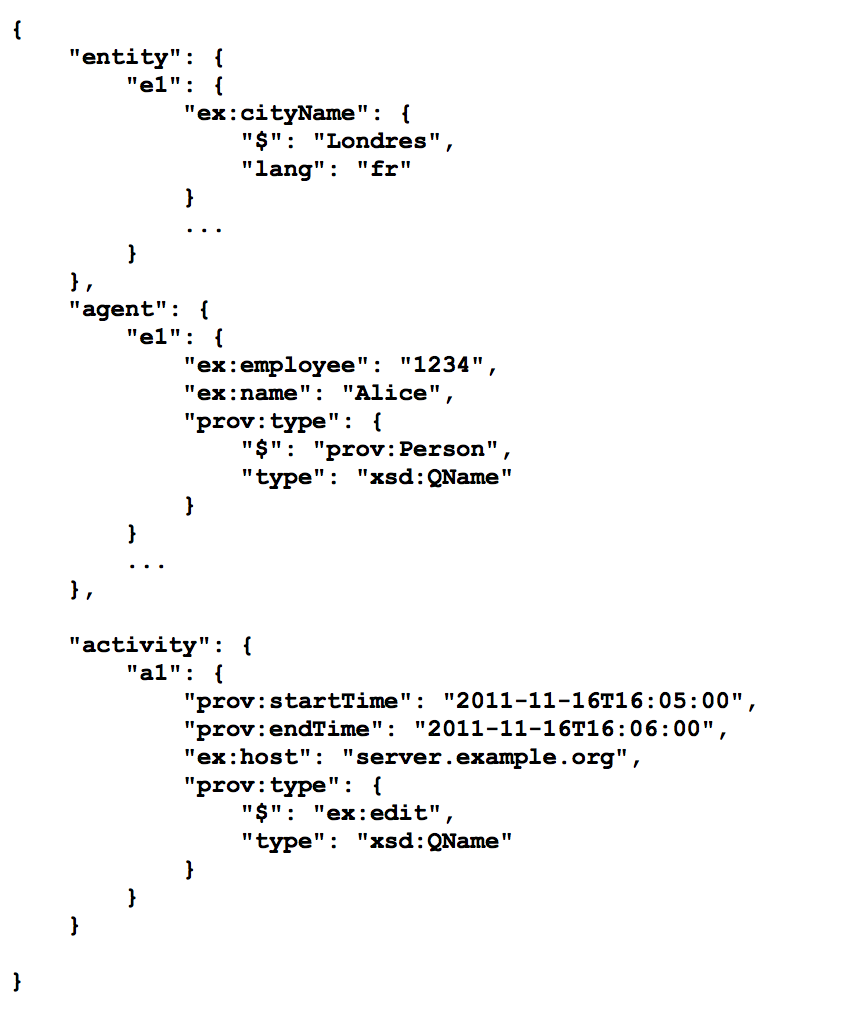
\includegraphics[height=5in]{prov_json.png}
\end{center}
\caption{PROV-JSON MODEL}

\end{figure}

\section{Overview of Data pruning techniques}

\subsection{Graph Compression}

\subsection{Dictionary Encoding}

\subsection{Arithmetic Encoding}


\section{Intrusion Detection for IoT}



%%% Local Variables: 
%%% mode: latex
%%% TeX-master: "thesis"
%%% End: 
